\section{Hash Functions}
\subsection*{Definition}
A hash function is a function $H:\{0,1\}^*\rightarrow \{0,1\}^{\ell}$ that
\begin{itemize}
    \item compresses long inputs into short (fixed-length) digests
    \item Is \emph{collision resistant}: Hard to find $x,x'$ s.t. $H(x)=H(x')$
\end{itemize}

(Keyed) Hash function with output length $\ell(n)$:
\begin{itemize}
    \item $\text{Gen}(1^n)$: Output a key $s$
    \item $H(s,x)$: $H^s(x)$ takes input $x\in\{0,1\}^*$ and outputs $H^s(x) \in \{0,1\}^{\ell(n)}$
\end{itemize}

Compression function: If input length is also fixed, i.e.,
 $x\in\{0,1\}^{\ell'}$ for some $\ell'>\ell$, then this 
 is called a compression function\\


Hash functions used in practice are a bit different:
\begin{itemize}
    \item Output length is fixed (e.g., 256-bits), not a function of $n$
    \item Usually used unkeyed
    \item Still generally believed to be collision resistant
\end{itemize}
  
\subsection*{Security Definition}
Let $\Pi=(\text{Gen,H})$ be a (keyed) hash function with output length $\ell$
$\text{Hash}-\text{Coll}_{\mathcal{A},\Pi}(n)$ is a game between an adversary $\mathcal{A}$
and a challenger:
\begin{itemize}
    \item The challenger chooses $s\leftarrow \text{Gen}(1^n)$ and sends it to $\mathcal{A}$
    \item $\mathcal{A}$ outputs two strings $(x,x')$
    \item $\text{Hash}-\text{Coll}_{\mathcal{A},\Pi}(n)=1$ (i.e.,$\mathcal{A}$ wins)
    if $H^s(x)=H^s(x')$
\end{itemize}
A hash function $\Pi=(\text{Gen},H)$ is \emph{collision resistant} if for all 
PPT $\mathcal{A}$ it holds that 
$\Pr[\text{Hash}-\text{Coll}_{\mathcal{A},\Pi}(n)=1]\le \text{negl}(n)$

\subsection*{Building a Hash Function}
\begin{itemize}
    \item Start with a compression function $h^s:\{0,1\}^{\ell'}\rightarrow \{0,1\}^{\ell}$
    \item Extend domain from $\ell'$ to arbitrary bit strings
\end{itemize}

Merkle-Damgard Domain Extension:\\
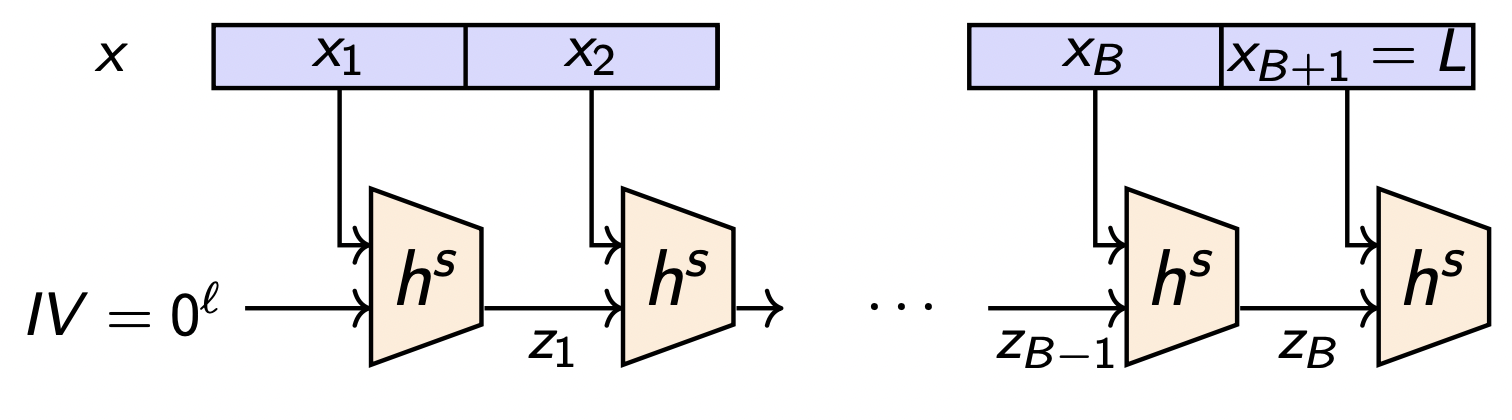
\includegraphics[width=\columnwidth]{Merkle-Damgard Domain Extension.png}
\begin{itemize}
    \item Let $h^s:\{0,1\}^{2\ell}\rightarrow \{0,1\}^{\ell}$ be 
    a compression function
    \item Given input $x\in\{0,1\}^L$
    \item Break $x$ into $\ell$ bit blocks
    \item Add length $L$ as last block
    \item Compute $H^s(x)$ as in the figure above
\end{itemize}
Proof of Collision Resistance: Show collision in $H^s$ gives collision in $h^s$
Suppose $x=(x_1,\cdots,x_B)$ and $x'=(x_1',\cdots,x_B')$ collide
$(H^s(x)=H^s(x'))$
\begin{itemize}
    \item Case 1: $L\neq L'$. $h^s(Z_B||L)=h^s(Z'_{B'}||L')$,
     but $L\neq L'\rightarrow \text{collision}$
    \item Case 2: $L=L'$. Find largest index where inputs to $h^s$ are different.
    Such index must exist since $x\neq x'$. At this index ,you have two different
    inputs to $h^s$ that produce same ouput $\rightarrow \text{collision}$
\end{itemize}

\subsection*{Application of Hash Functions}
Storing password with salt:
\begin{itemize}
    \item $U$ creates $pwd$ when registering for site
    \item Site chooses salt $s\leftarrow \{0,1\}^n$, computes $H(s||pwd)$ and
    stores $(\text{ID},s,H(s||pwd))$
    \item When logging in, user enters $pwd'$, server finds $s$, computes
    $H(s||pwd')$ and checks password file
\end{itemize}

Merkle Tree:\\
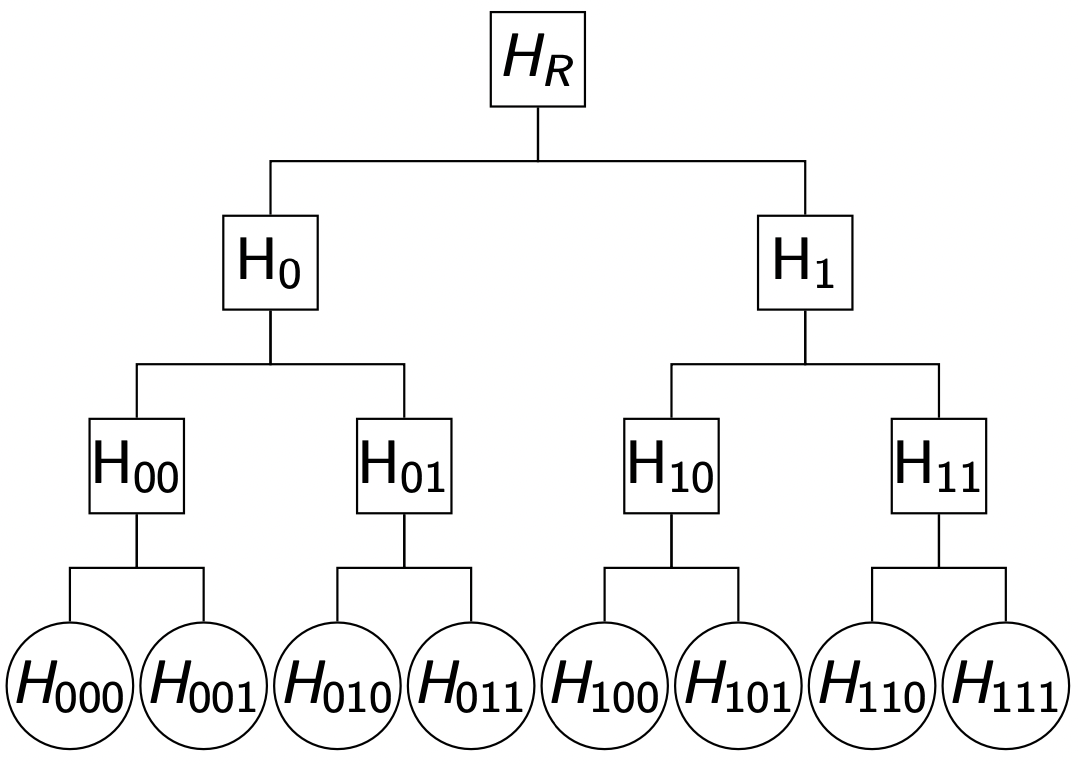
\includegraphics[width=\columnwidth]{Merkle Tree.png}
\begin{itemize}
    \item $U$ has files $x_{000},\cdots,x_{111}$, computes $H_{000}=H(x_{000}),\cdots$
    \item $H_{00}=H(H_{000},H_{001}), \cdots$
    \item $U$ does the same for all levels
    \item $U$ stores $H_R$ and uploads all files to $S$
    \item $U$ downloads $x_{001}$ and wants to check it's correct
    \item $S$ sends $U$ all sibling hashes along to the path to root:
    $H_{000},H_{01},H_1$
    \item $U$ computes $H_{001}$ and can now recompute up to $H_R$
\end{itemize}

\subsection*{Domain Extension for MACs(Hash-and-MAC)}
Building blocks:
\begin{itemize}
    \item $\Pi=(\text{Gen,Mac,Verify})$: Secure MAC for $\ell(n)$ bit messages
    \item $\Pi_H=(\text{Gen}_H,H)$: CRHF with output length $\ell(n)$
\end{itemize}
construct $\Pi'=(\text{Gen}',\text{Mac}',\text{Verify}')$:
\begin{itemize}
    \item $\text{Gen}'(1^n)$: Choose $k\leftarrow \text{Gen}(1^n)$,
    $s\leftarrow \text{Gen}_H(1^n)$, output $k'=(k,s)$
    \item $\text{Mac}'_{k'}(m)$: output $t=\text{Mac}_k(H^s(m))$
    \item $\text{Verify}'_{k'}(m,t)$: output 1 if $t=\text{Mac}_k(H^s(m))$
\end{itemize}

\subsection*{HMAC}
$\text{Mac}_{s,k}(m)$:
Output $t=H^{s}((k\oplus opad)||H^s((k\oplus ipad)||m))$
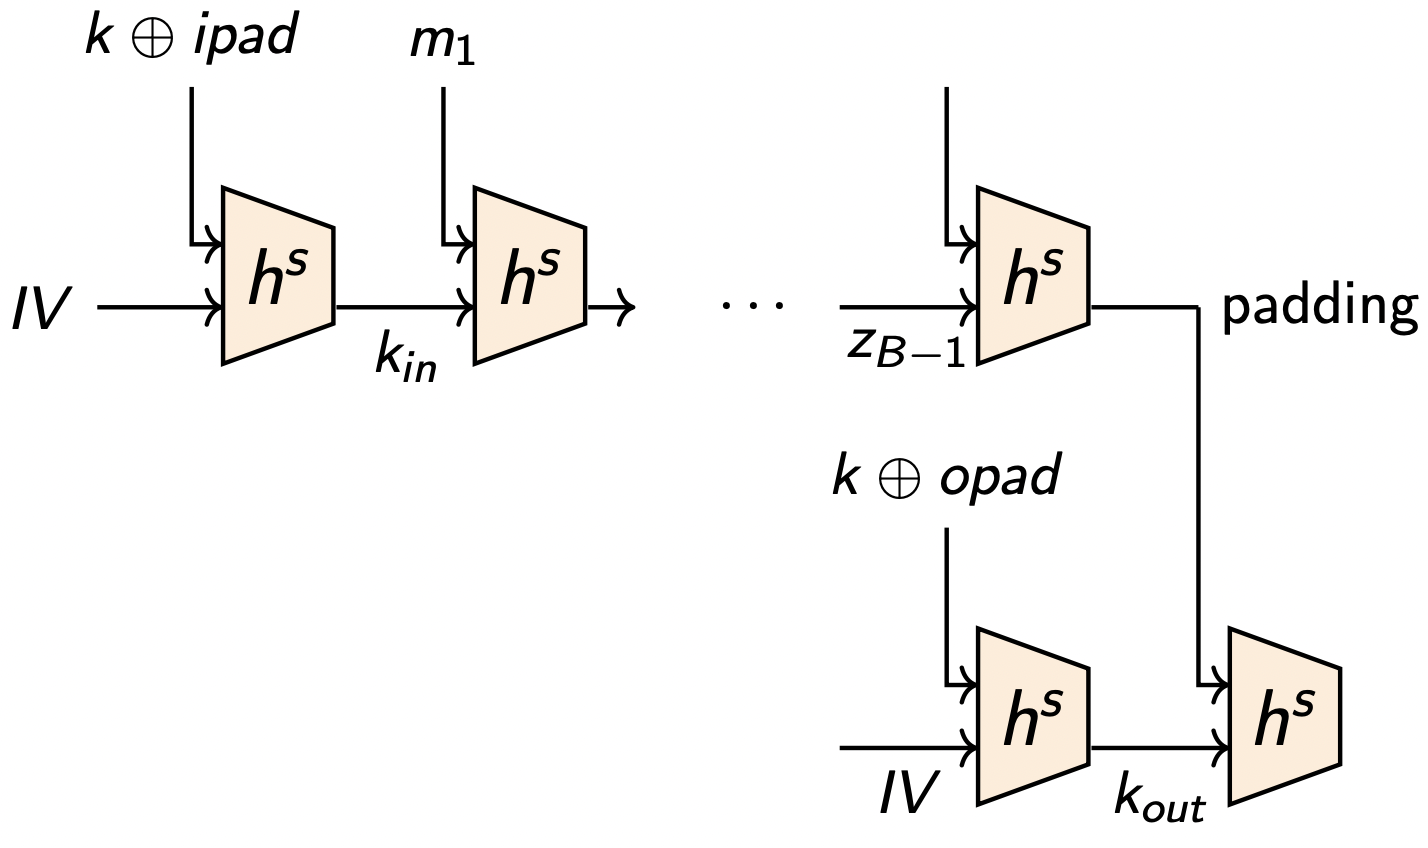
\includegraphics[width=\columnwidth]{HMAC.png}